\documentclass[border=10pt]{standalone}
\usepackage{pgfplots}
\pgfplotsset{compat=1.18}
\begin{document}
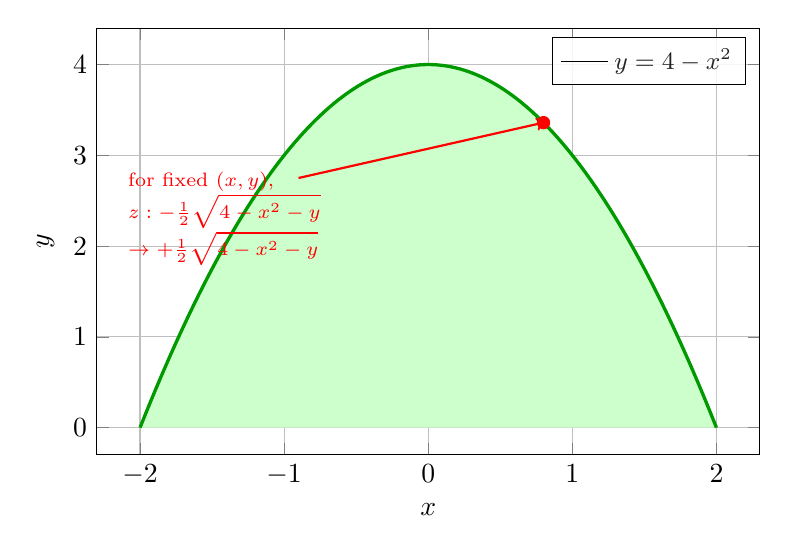
\begin{tikzpicture}
\begin{axis}[
    xmin=-2.3, xmax=2.3, ymin=-0.3, ymax=4.4,
    xlabel=$x$, ylabel=$y$,
    width=10cm, height=7cm,
    grid=both,
    clip=false,
    legend style={at={(0.98,0.98)}, anchor=north east, font=\small, fill=white, fill opacity=0.85},
]
\addplot[fill=green!20, draw=none, domain=-2:2, samples=120] {4-x^2} \closedcycle;
\addplot[green!60!black, very thick, domain=-2:2, samples=120] {4-x^2};
\addlegendentry{$y=4-x^2$}
\addplot[only marks, mark=*, red, mark size=2.2pt, forget plot] coordinates {(0.8,3.36)};
\draw[red, ->, thick] (axis cs:-0.9,2.75) -- (axis cs:0.8,3.36);
\node[red, anchor=west, font=\scriptsize, align=left] at (axis cs:-2.15,2.3)
    {for fixed $(x,y)$,\\ $z:-\frac{1}{2}\sqrt{4-x^2-y}$\\ $\to+\frac{1}{2}\sqrt{4-x^2-y}$};
\end{axis}
\end{tikzpicture}
\end{document}
